% Document class, language and encoding setup
\documentclass[a4paper,12pt,danish]{article}

\usepackage[danish]{babel}
\usepackage[latin1]{inputenc}
\usepackage[T1]{fontenc}
% Fixing the font issue
\usepackage{ae,aecompl}

% Color package
\PassOptionsToPackage{dvipsnames}{xcolor}
	\RequirePackage{xcolor} % [dvipsnames] 
	
% Allows page-links in pdf file
\usepackage[colorlinks=true]{hyperref}

% Allows commands to emit a space "at the end"
\usepackage{xspace}

% Listings setup
\usepackage{listings}

% Graphics setup
\usepackage{graphicx}

% Tikz til spiderweb diagram
\usepackage{tikz}
\usetikzlibrary{shapes}

\newcommand{\D}{5} % number of dimensions (config option)
\newcommand{\U}{5} % number of scale units (config option)

\newdimen\R % maximal diagram radius (config option)
\R=4cm 
\newdimen\L % radius to put dimension labels (config option)
\L=4.7cm

\newcommand{\A}{360/\D} % calculated angle between dimension axes  

\begin{document}

\begin{titlepage}
\newcommand{\HRule}{\rule{\linewidth}{0.5mm}}

\begin{center}

\HRule \\[0.5cm]
\textsc{ \Huge SOE mini-projekt}\\[0.3cm]

\HRule \\[1cm]

\textsc{\Large SW505E13 \\ 3.1.12}\\[0.5cm]

{\large
Anders Roland Nielsen \\
Bruno Thalmann \\
Mikael Elki�r Christensen \\
Mikkel Sand� Larsen \\
Stefan Marstrand Getreuer Micheelsen \\
Stefan Thilemann
}

\vfill

{\large Aalborg Universitet --- 22. november, 2013}

\end{center}

\end{titlepage}

\tableofcontents

% INCLUDE WORKSHOPS HERE ==========>
\chapter{Udviklingsmetode}\label{udviklingsmetode}
% Document class, language and encoding setup
\documentclass[a4paper,12pt,danish]{article}

\usepackage[danish]{babel}
\usepackage[latin1]{inputenc}
\usepackage[T1]{fontenc}
% Fixing the font issue
\usepackage{ae,aecompl}

% Color package
\PassOptionsToPackage{dvipsnames}{xcolor}
	\RequirePackage{xcolor} % [dvipsnames] 
	
% Allows page-links in pdf file
\usepackage[colorlinks=true]{hyperref}

% Allows commands to emit a space "at the end"
\usepackage{xspace}

% Listings setup
\usepackage{listings}

% Graphics setup
\usepackage{graphicx}

% Tikz til spiderweb diagram
\usepackage{tikz}
\usetikzlibrary{shapes}

\newcommand{\D}{5} % number of dimensions (config option)
\newcommand{\U}{5} % number of scale units (config option)

\newdimen\R % maximal diagram radius (config option)
\R=4cm 
\newdimen\L % radius to put dimension labels (config option)
\L=4.7cm

\newcommand{\A}{360/\D} % calculated angle between dimension axes  

\begin{document}

\begin{titlepage}
\newcommand{\HRule}{\rule{\linewidth}{0.5mm}}

\begin{center}

\HRule \\[0.5cm]
\textsc{ \Huge SOE Mini-projekt 1 \\ \Large Udviklingsmetode}\\[0.3cm]

\HRule \\[1cm]

\textsc{\Large SW505E13}

\vfill

{\large Efter�rssemesteret 2013}

\end{center}

\end{titlepage}

\section{Beskrivelse af projekt}
Projektet handler om udvikling af en metode til autonom mapping, vha. en \legoms NXT\textregistered-robot, med kendt position ved brug af en \mskinect til lokalisering.

\section{Den valgte udviklingsmetode}\label{valgtmetode}
I projektperioden har gruppen valgt at arbejde med en metode der tager udgangspunkt i SCRUM, men samtidig benytter elementer fra XP.

Valget er prim�rt truffet ud fra den problemstilling vi som studerende st�r overfor i forbindelse med et semester projekt; alts� at der skal produceres b�de en rapport og k�rende software.
Det er gruppens vurdering at XPs prim�re styrker ligger i programmeringsfasen, men halter i forhold til rapportskrivning.
Dele af XP er derfor tilvalgt for at st�tte op om metoden anvendt til programmering.

I det f�lgende afsnit vil vi beskrive de metoder vi har unders�gt, samt begrunde vores valg af metode.

\subsection{Boehms stjerne-model}
Til at hjælpe med valg af udviklingsmetode er der taget udgangspunkt i Boehms stjerne-model\cite{boehm}.
Modellen beskriver projektgruppens arbejdsform ud fra fem faktorer.
Herunder gennemgås disse faktorer og der gives en vurdering af gruppen i relation til disse.
Gruppens vurderinger er plottet på \cref{boehms:stjerne}.
{
\newcommand{\D}{5} % number of dimensions (config option)
\newcommand{\U}{5} % number of scale units (config option)
\newcommand{\UU}{50}

\newdimen\R % maximal diagram radius (config option)
\R=3.5cm 
\newdimen\L % radius to put dimension labels (config option)
\L=3.7cm

\newcommand{\A}{360/\D} % calculated angle between dimension axes  

\begin{figure}[h]
\centering
\begin{tikzpicture}[scale=1]
  \path (0:0cm) coordinate (O); % define coordinate for origin

  % draw the spiderweb
  \foreach \X in {1,...,\D}{
    \draw (\X*\A+90:0) -- (\X*\A+90:\L);
  }

  \foreach \Y in {0,...,\U}{
    \foreach \X in {1,...,\D}{
      \path (\X*\A+90:\Y*\R/\U) coordinate (D\X-\Y);
      \fill (D\X-\Y) circle (1pt);
    }
%    \draw [opacity=0.3] (90:\Y*\R/\U) \foreach \X in {1,...,\D}{
%        -- (\X*\A+90:\Y*\R/\U)
%    } -- cycle;
  }
  \foreach \X in {1,...,\D}{
    \path (\X*\A+90:5.7*\R/\U) coordinate (D\X-T);
  }
  \foreach \Y in {0,...,\UU}{
    \foreach \X in {1,...,\D}{
      \path (\X*\A+90:\Y*\R/\UU) coordinate (D\X--\Y);
    }
  }
  
  \path (D5-T) node (L1) {\scriptsize Personnel};
  \draw (D5-5) node[left] {\tiny (1A/1B) 100};
  \draw (D5-5) node[right] {\tiny 0 (2/3)};
  \draw (D5-4) node[left] {\tiny 75};
  \draw (D5-4) node[right] {\tiny 25};
  \draw (D5-3) node[left] {\tiny 50};
  \draw (D5-3) node[right] {\tiny 50};
  \draw (D5-2) node[left] {\tiny 25};
  \draw (D5-2) node[right] {\tiny 75};
  \draw (D5-1) node[left] {\tiny 0};
  \draw (D5-1) node[right] {\tiny 100};
  
  \path (D4-T) node (L2) {\scriptsize Dynamism};
  \draw (D4-5) node[below] {\tiny 1};
  \draw (D4-4) node[below] {\tiny 5};
  \draw (D4-3) node[below] {\tiny 10};
  \draw (D4-2) node[below] {\tiny 30};
  \draw (D4-1) node[below] {\tiny 50};
  
  \path (D3-T) node (L3) {\scriptsize Culture};
  \draw (D3-5) node[left] {\tiny 10};
  \draw (D3-4) node[left] {\tiny 30};
  \draw (D3-3) node[left] {\tiny 50};
  \draw (D3-2) node[left] {\tiny 70};
  \draw (D3-1) node[left] {\tiny 90};
  
  \path (D2-T) node (L4) {\scriptsize Size};
  \draw (D2-5) node[right] {\tiny 300};
  \draw (D2-4) node[right] {\tiny 100};
  \draw (D2-3) node[right] {\tiny 30};
  \draw (D2-2) node[right] {\tiny 10};
  \draw (D2-1) node[right] {\tiny 3};
  
  \path (D1-T) node (L5) {\scriptsize Criticality};
  \draw (D1-5) node[below, align=center, font=\tiny] {Many\\Lives};
  \draw (D1-4) node[above, align=center, font=\tiny] {Single\\Life};
  \draw (D1-3) node[below, align=center, font=\tiny] {Essential\\Funds};
  \draw (D1-2) node[above, align=center, font=\tiny] {Discretionary\\Funds};
  \draw (D1-1) node[below, align=center, font=\tiny] {Comfort};
    
  \draw [color=blue,line width=1.5pt,opacity=0.5]
    (D1--10) --
    (D2--14) --
    (D3--15) --
    (D4--40) --
    (D5--10) -- cycle;

\end{tikzpicture}
\caption{Boehms stjerne-model}
\label{boehms:stjerne}
\end{figure}
}

\begin{description}
\info{Personnel}{beskriver projektgruppens medlemmers ''niveau'' i relation til programmering.
Denne inddeling sker efter Cockburns skala \cite[Tabel 2]{boehm}, der beskriver niveau i relation til det der skal produceres.}
{Vi har i projektgruppen vurderet at alle gruppens medlemmer er på niveau 2 eller 3.}

\info{Dynamism}{angiver i hvilken grad det forventes at der opstår ændringer i et projekts kravspecifikation.
Det fortæller altså i hvilken grad projektgruppen skal være i stand til at tilpasse sig forandringer i krav.}
{Da vi arbejder problembaseret, tages der udgangspunkt i nogle simple og konkrete krav, der i løbet af projektperioden kun vil blive yderligere præciseret.}

\info{Culture}{er en vurdering af hvorvidt en projektgruppes medlemmer trives bedst med kaos eller orden.
På skalaen angives ''hvor meget'' kaos gruppen trives med.}
{Projektgruppens medlemmer har hver især vurderet hvor de ligger på skalaen.
Gennemsnittet af disse vurderinger er på 69,2\%.}

\info{Size}{udtaler sig udelukkende om størrelsen på den gruppe der skal arbejde på et projekt.}
{Projektgruppen består af 6 personer.}

\info{Criticality}{beskriver ''hvor vigtigt'' det er at det endelige produkt er fungerende og lever op til alle krav.
Skalaen angiver denne vigtighed i form af hvilken effekt det har hvis dette ikke er tilfældet.}
{Da den robot, som er projektets mål, ikke skal sættes i produktion, vil den aldrig have højere betydning end \textbf{Comfort} på skalaen.
Det er naturligvis et mål for projektgruppen at have en fungerende robot ved semestrets afslutning.
Men da den tekniske forståelse, som er et biprodukt af det udviklede, ligeledes udbygges, vurderer vi det ikke som kritisk hvis robotten ikke er fuldt fungerende.}
\end{description}

Ud fra modellen (\cref{boehms:stjerne}) ses det at projektgruppen med fordel kan vælge en agil metode til projektarbejdet, da plottet ligger nærmest midten for næsten alle punkter.
Det eneste punkt der ikke direkte anbefaler en agil tilgang er \emph{Dynamism}.
Dog påpeger Boehm og Turner \cite[side 2]{boehm} at dette ikke er et problem:
\quoter{Boehm og Turner}{``For Dynamism, agile methods are at home with 
both high and low rates of change, but plan-driven 
methods prefer low rates of change.''} 
Altså har få krav ikke betydning for valget mellem en agil og en traditionel metode.
Vi kan nu skifte fokus til valg af en specifik agil metode.
I det følgende afsnit gives en kort beskrivelse af udvalgte agile metoder.
\subsection{Eksisterende metoder}\label{existing}
Til at finde en passende udviklingsmetode til projektgruppen er der kigget p� f�lgende eksisterende agile metoder: SCRUM, XP og UP.\cite{larman}
Der er kun kigget netop disse metoder, da de er blevet pr�senteret i \emph{Software Engineering} kurset som v�rende meget udbredte metoder.
Vi kan derfor med fordel v�lge en af disse metoder til vort studieprojekt.


\paragraph{XP} er en agil metode der tager udgangspunkt i at de udviklere der er i gruppen har et h�jt fagligt niveau.
Med det udgangspunkt frav�lges en r�kke elementer fra plandrevet udvikling der ikke giver kunden direkte v�rdi.
P� et semesterprojekt har vi ikke en egentlig kunde at udvikle til, hvilket p�virker afvejningen af hvad der skaber v�rdi.
Samtidig er vi i en l�ringsproces hvor den bagved liggende teori er af stor relevans, og skal dokumenteres i form af en rapport.
Derfor har vi fravalgt XP som overordnet metode, men vil i \cref{ourmethod} ``\nameref{ourmethod}'' beskrive nogle af de elementer vi inkluderer til programmering.

\paragraph{UP} er en ligeledes en agil metode til software udvikling.
UP er dog baseret p� st�rre teams med udskiftning og sikrer via forskellige typer dokumentation at denne udskiftning er mulig.
Eftersom det ``team'' vi arbejder i, i form af projektgruppen, kun er p� seks mand og derfor ikke s�rlig stort (jf. \cref{boehms:stjerne}) og helt uden udskiftning har vi helt fravalgt UP.
Vi ser desuden ogs� p� Boehms model at der er en h�j grad af kaos hvilket strider mod den rigide dokumentation i UP.

\paragraph{SCRUM} stemmer godt overens med projektet, da den er meget fleksibel og nem at tilpasse.

{ %Der anvendes curly brackets til at lave lokal kommando

\newcommand{\XPhere}{\marginpar{\textbf{\footnotesize XP}}}

\section{Vores metode}\label{ourmethod}
Vi har valgt at tage udgangspunkt i SCRUM (jf. \cref{existing}) og derudover inddrage elementer fra XP til is�r at styrke programmeringsprocessen.
I dette afsnit vil implementationen af vores udviklingsmetode blive pr�senteret, og hvor det er n�dvendigt vil begrundelsen for et valg blive givet.

\subsection{Roller}
SCRUM arbejder med et s�t roller, der typisk tildeles bestemte personer.
I kraft af at dette projekt er et semesterprojekt, laver vi nogle s�rlige udgaver af disse roller.
Herunder beskrives og tildeles de forskellige roller.
\begin{description}
\info{Product owner}
{har ansvaret for at bestemme fokus for projektet.
Product owner skal prioritere opgaver ved planl�gning af et sprint og vurdere om det der produceres kan anvendes eller ej.}
{Eftersom produktet af dette semester projekt ikke udvikles til en kunde eller med en bestemt kunde i tankerne, findes der ikke en udenforst�ende til at varetage denne rolle.
Gruppen p�tager sig selv rollen og foretager prioritering/vurdering ud fra studieordningen og projektets problemformulering.}

\info{Scrum master}
{s�rger for at gruppen arbejder produktivt, med udgangspunkt i SCRUM v�rdier.}
{Denne rolle tildeles et nyt gruppemedlem i starten af hvert sprint, s�ledes at alle gruppens medlemmer p� skift p�tager sig rollen.
Gruppen anvender denne model for at alle medlemmer kan fors�ge sig i rollen.


Scrum masterens opgave er at starte og dirigere morgen-, sprint- og vejlederm�der.}

\info{Team}
{beskriver det team der arbejder p� et givent projekt og stiller en r�kke krav til teamets medlemmer.}
{Da projektet udvikles af en studiegruppe best�r teamet af en fast gruppe p� 6 mand; alle med evner til at udf�re alle mulige arbejdsopgaver.}
\end{description}

\subsection{Ceremonier}

Der vil blive k�rt sprints af l�ngden 1 uge.
Dette menes som en uge i time-antal for at tage h�jde for forel�sninger og andet der begr�nser projekt-tiden i en given uge.
Timeantallet for et sprint er 36 timer og er bestemt ud fra at vi arbejder 8 timer om dagen undtagen fredag hvor der regnes med 4 timer pga. \nameref{friday_meeting} som specificeret i \cref{friday_meeting}.
I l�bet af et sprint vil f�lgende ceremonier v�re en del af processen.
\\
\subsubsection{Sprint planl�gningsm�de}
Sprint planl�gningsm�det foreg�r inden hvert sprint. 
Der planl�gges hvilke stories der tages med til det n�ste sprint. 
Disse stories skal beskrive de krav projektet har.
Stories bliver lavet ud fra projektets problemformulering og studieordningen.
Disse stories prioriteres efter hvor vigtige de er for slutproduktet.

Opgaver diskuteres s� det er klart hvilke krav opgaven indeholder, samt hvorn�r opgaven er l�st.
Der spilles planning poker om hver enkelt opgave.
Hvis en opgave er for stor bliver den opdelt i mindre opgaver.
Der spilles planning poker indtil alle opgaver vurderes til at kunne l�ses inden for 2 dage som er det scrum\cite{larman} anbefaler.

\subsubsection{Morgenm�de}
Hver morgen kl. 08.15 (s�fremt der ikke er forel�sning) vil der blive holdt et morgenm�de, hvor der for hvert gruppemedlem vil blive givet f�lgende status:
\begin{itemize}
\item{Er der nogen der skal g� f�r tid i dag?}
\end{itemize}
Derefter bliver hver enkelt person spurgt af Scrum Masteren:
\begin{enumerate}
\item{Hvad lavede du i g�r?}
\item{Hvad skal du lave i dag?}
\item{Er der noget i vejen?}
\end{enumerate}
I forbindelse med dette opdaterer hvert gruppemedlem scrumboardet.

\subsubsection{Sprint vurdering}
Sprint vurdering indledes med at ridse op hvad det netop afsluttede sprint indeholdte. 
Hvert gruppemedlem freml�gger derefter kort de resultater de har opn�et i sprintet.
Forberedelsestiden til freml�ggelsen er maks. 15 min.

\subsubsection{Fredagsm�de}\label{friday_meeting}
Hver fredag holdes et fredagsm�de, hvis form�l er at identificere og udbedre eventuelle sociale problemer i gruppen.
Fredagsm�det styres af scrum masteren som f�lger en specifik dagsorden, der blandt andet indeholder sp�rgsm�l som: ``Hvordan g�r det'' og ``konsruktiv kritik til andre gruppemedlemmer. 
Fredagsm�det har samtidig til form�l at v�re en afslappet og social afslutning p� ugen.

\subsection{Praksis fra XP}\label{method:xp:practice}
Som n�vnt i \cref{ourmethod} har vi udvalgt nogle praksisser fra XP, som vi vil benytte i forbindelse med programmeringsopgaver.
Disse praksisser vil her blive beskrevet kort.

\paragraph{Simple design}
Ved l�sning af en opgave v�lges den mest simple l�sning, s� der fokuseres p� at f� l�st kerneproblemet.

\paragraph{Refactoring}
Kodebasen vil l�bende blive refaktoriseret for at eliminere duplikeret kode samt for at forsimple og/eller forbedre det eksisterende.
%Der vil l�bende blive udf�rt refaktoriset kode s� dublikeret kode fjernes og koden generelt bliver forsimplet eller forbedret.

\paragraph{Pair programming}
Gruppen vil fors�ge at bruge denne praksis i situationer hvor der er f� programmeringsopgaver, men ikke som en generel praksis.

\paragraph{Collective ownership}
Det er gruppens filosofi at alle ejer b�de kode og rapport, hvorfor alle kan lave �ndringer hvis det vurderes n�dvendigt.

\paragraph{Sustainable pace}
Sprints er bestemt til at vare en uge for at holde et konsistent tempo dvs. at arbejde overtid ikke er tilladt.
Dette g�r det ogs� lettere at planl�gge sprints.

\paragraph{Code standards}
For at ensarte koden har gruppen fastsat en r�kke kodestandarder der skal overholdes.

\todo[inline]{Jeg synes der mangler en generel afrunding af hele rapporten. Det slutter lidt brat. Mvh. Thilemann.}

\begin{thebibliography}{9}

\bibitem{boehm}
  Boehm, B.; Turner, R., ''Observations on balancing discipline and agility'', Agile Development Conference, 2003.
  ADC 2003. Proceedings of the , vol., no., pp.32,39, 25-28 June 2003
  
\bibitem{larman}
Larman, Craig., ''Agile and Iterative Development: A Manager's Guide''.
Addison-Wesley, 2004.

\bibitem{checklist}
Gloger, Boris, ``Scrum Checklist'', 

``http://sict.moodle.aau.dk/file.php/797/General\_Course\_Materials/
literature/Scrum\_CheckList\_2011.pdf'', set 10 Oktober 2013
\end{thebibliography}

\end{document}
\chapter{V�rkt�jer og teknikker}
\section{SWOT analyse}\label{swot:analyse}
I dette kapitel er projektet analyseret i forhold til dets styrker, svagheder, muligheder og trusler (SWOT analyse), for at give et overblik over projektes indre form�en (styrker og svagheder), men ogs� for at belyse de elementer som kan p�virke projektet positivt og negativt (muligheder og trusler).

V�rkt�jer der allerede er inddraget i projektet er ikke beskrevet, p� trods af at dette kapitel beskriver v�rkt�jer og teknikker.
Dette valg er taget p� baggrund af �nsket om at unders�ge nye v�rkt�jer som kan styrke projektarbejdet yderligere.

\subsection{Styrker \textnormal{(\textbf{S}trengths)}}

\paragraph{Mere end �t grupperum}
Det ses som en fordel at gruppen er blevet tildelt et ekstra grupperum, da det giver bedre mulighed for at teste robotten i et testmilj�.
Det fjerner desuden ogs� st�j fra det ''rigtige'' grupperum, s�ledes der kan arbejdes mere koncentreret.

\paragraph{Egen udviklingsmetode}
Det er en styrke at gruppen har dets egen udviklingsmetode tilpasset til gruppens behov og projekt.
Den er beskrevet i \cref{udviklingsmetode}.

\paragraph{Matematisk baggrund}
Det anses som en fordel at alle i gruppen besidder en form for matematisk baggrund (gymnasie, HTX osv.).

\paragraph{Veldefinerede minimumsm�l for projektet}
Gruppen har fundet god enighed omkring m�lene for projektet; disse er endvidere defineret i form af diverse ''stories'' som beskriver en overordnet funktionalitet af det endelige produkt.
Dette koblet sammen med det initierende problem giver et godt samlet udtryk af hvad der skal arbejdes hen imod.

\paragraph{Godt samarbejde mellem gruppens medlemmer}
Der er i gruppen kun ganske f� konflikter (navnligt n�r der diskuteres essentielle emner i forhold til fremtidig retning af projektet).
Der forefindes ogs� en gruppekontrakt der respekteres af alle gruppens medlemmer, hvilket fremmer konfliktl�sning.

\paragraph{God arbejdsmoral}
Der er i gruppen stor enighed om hvorn�r der skal holdes pause eller ej.
Derudover arbejdes der efter bestemte arbejdstider, som overholdes af alle gruppens medlemmer.
Alt arbejde foreg�r ogs� i grupperummene, hvilket g�r det nemt at stille sp�rgsm�l til andre gruppemedlemmer.

\paragraph{F� sygedage}
Der er kun afholdt ganske f� sygedage, hvilket fremmer gruppearbejdet.

\subsection{Svagheder \textnormal{(\textbf{W}eaknesses)}}

\paragraph{Manglende viden omkring MI}\label{swot:manglende_viden_mi}
Dette anses som v�rende en af gruppens st�rste svagheder; dog er det forventeligt, da ingen i gruppen f�r har arbejdet med Maskin Intelligens (eller sandsynligheder) og at kurses indhold pr�senteres l�bende.

\paragraph{Usikkerhed pga. l�bende optagelse af viden}\label{swot:optagelse_af_viden}
H�nger delvist sammen med ovenst�ende, da ikke alt indhold i kurserne pr�senteres i den r�kkef�lge der n�dvendigvis er mest relevant i forbindelse med projektets fremgang.

\paragraph{Forskelligt niveau/kvalitet af kode}\label{swot:niveau_af_kode}
P� trods af at alle gruppens medlemmer skriver kode af fornuftig kvalitet, s� er der stadig forskel p� medlemmers erfaring og hvilken type sprogkonstruktioner der benyttes.
Dette kan g�re noget kode sv�rt l�seligt for nogle og kan dermed ogs� f� betydning for kvaliteten n�r al kode samles.

\paragraph{Kode retningslinjer - bad smells}\label{swot:bad_smells}
Gruppekontrakten indeholder diverse retningslinjer for kode; det er dog ikke altid muligt at fjerne alle ''bad smells'', da alle koder forskelligt.
Gruppekontrakten skal fjerne de st�rste uenigheder.
Mindre forskelle kan tolereres -- s�l�nge koden er velskrevet og l�selig.

\subsection{Muligheder \textnormal{(\textbf{O}pportunities)}}

\paragraph{Hj�lpsom og engageret vejleder}
Dette punkt anses som v�rende af essentiel kvalitet for hele projektets fremgang. 
Da gruppen har arbejdet sammen om flere projekter og derfor ogs� med flere vejledere, findes der store muligheder i at nuv�rende vejleder engagerer sig 100 procent i projektarbejdet.
Dette er med til at skubbe projektet i den rigtige retning og g�r det ligeledes muligt at holde fokus p� studieordningens m�l.

\paragraph{Kontakt til andre grupper}
Det findes v�rdi i muligheden for at tage kontakt til andre projektgrupper som arbejder med en lignende problemstilling som dette projekt.
St�der vi p� et problem og konkluderer at det ikke kan l�ses med den viden vi har tilegnet os, kan de andre grupper med fordel bes�ges for at f� id�er til en videre l�sning.

\paragraph{Adgang til udstyr}
Det anses af gruppen at v�re en stor mulighed at der stilles diverse udstyr tilr�dighed af universitetet.
Desuden er det ogs� nemt og hurtigt at fremskaffe nyt/alternativt udstyr, hvis der pludselig opst�r mangler.

\paragraph{Ny viden}\label{swot:ny_viden}
Der findes store muligheder i at tilegne sig ny og relevant viden is�r via kurser, men ogs� andet eksternt materiale.
S�ledes vil b�ger, artikler, internettet og generelt som mange kilder som muligt, blive inddraget i informationss�gning (og delt i gruppen).
Dette kan s�tte projektet i et nyt perspektiv og afhj�lpe fremtidigt arbejde.

\paragraph{Git Issues}
Da b�de vores rapport(er) og kode for projektet er versionsstyret (via \url{http://github.com}), er der mulighed for at benytte en funktionalitet de kalder for ''Git Issues''.
Dette er en avanceret form for todo-notes som f�lger hvert enkelt commit.
Det g�r det muligt at oprette et problem (s�kaldt \textit{issue}), hvis man finder fejl i kode.
Dette kan h�jne kvaliteten af projektet, da det giver en overisgt over de problemer der skulle v�re.

\subsection{Trusler \textnormal{(\textbf{T}hreats)}}

\paragraph{Misforst�ede l�ringsm�l}\label{swot:laeringsmaal}
Der er i studieordningen fundet et afsnit der siger at man i dette projekt skal kunne fremvise et k�rende indlejret system.
Dette har givet anledning til forvirring, da der andetsteds st�r at der blot skal inddrages relevant teori fra de forskellige kurser, hvilket i vores tilf�lde er MI (maskin intelligens).
Da der ikke har v�ret fokus p� at bygge et indlejret system, men derimod et intelligent system, har dette aspekt manglet i vores l�sning.
Det er efterf�lgende blevet besluttet at bygge en mindre del af l�sningen som et indlejret system, men dette aspekt anses stadig som en trussel, da der endnu ikke forefindes en endelig afklaring.

\paragraph{Vejleder skifter mening undervejs}\label{swot:vejleder}
P� trods af at vi er meget tilfredse med vejleder samarbejdet, anses det stadig som en trussel hvis han skulle skifte mening undervejs.
Dette kan betyde at v�sentlige m�ngder arbejde er spildt, hvilket i sidste ende kan betyde at vores tidsplan ikke holder.


\section{Udvalgte v�rkt�jer og teknikker}
Efter granskningen af SWOT analysen, som beskrevet i \cref{swot_analyse}, er det besluttet at vi vil fokusere p� at arbejde med design patterns, da disse kan tilf�je h�j v�rdi i forhold til de problemer der er fundet med SWOT analysen.
Da gruppen i forvejen kender til mange forskellige typer v�rkt�jer og allerede har inddraget mange i projektarbejdet (elementer fra SCRUM, Xtreme Programming, Git versionsstyring m.m.), ses design patterns som en god udfordring, da det er et element som ikke f�r har v�ret inddraget i udviklingsforl�bet.
F�lgende afsnit (\cref{design_patterns_beskrivelse}) fokuserer s�ledes p� at beskrive hvad design patterns er.

\subsection{Design Patterns}\label{design_patterns_beskrivelse}

\section{Rationale for valg}
I dette afsnit vil der være en begrundelse af de valgte værktøjer.
Værktøjerne er valgt på baggrund af SWOT analysen præsenteret i \cref{swot:analyse}.

\subsection{Design Patterns}\label{workshop2:designpatterns}
Design patterns er valgt pga. følgende punkt i SWOT analysen:
\begin{itemize}
\item Forskelligt niveau/kvalitet af kode (\cref{swot:niveau_af_kode})
\end{itemize}

Som man kan se på de ovenståeden punkter skal design patterns være med til at hæve niveauet for koden og ensrette forståelsen af den.
Det skal være med til at fjerne nogle af de ''bad smells'' der kan forekomme.
Hvis alle bruger design patterns, vil det blive nemmere at læse, og derefter også reaktorfere koden for andre.

\subsection{Risk Management}
Risk Management er valgt pga. følgende punket i SWOT analysen:

\begin{enumerate}
\item Manlgende viden omkring MI (\cref{swot:manglende_viden_mi})
\item Usikkerhed pga. løbende optagelse af viden (\cref{swot:optagelse_af_viden})
\item Misforståede læringsmål (\cref{swot:laeringsmaal})
\item Vejleder skifter mening undervejs (\cref{swot:vejleder})
\end{enumerate}

Som det kan ses på de ovenstående punkter er det en meget god ide at lave risk management med de risikoer hvert punkt indeholder.
Men da det tager lang tid at lave risk management, og der er begrænset tid til projektet, er det fravalgt da det vurderes at afkastet ikke står mål med indsatsen det vil kræve.
\section{Implementations strategi}
For at kunne implementere design patterns i gruppens projektarbejde, vil vi s�ge at �ge gruppemedlemmernes kendskab til forskellige design patterns.
Dette skal v�re med til at sikre, at alle gruppens medlemmer har det forn�dne kendskab til design patterns.
Som v�rkt�j til at f� denne viden afholder gruppen en design pattern workshop.
M�let med denne er at foretage vidensdeling om forskellige design patterns.
For at kunne g�re dette, er det n�dvendigt f�rst at fastsl� hvilke design patterns gruppen v�lger at fokusere p�.
Til dette har gruppen valgt at tage udgangspunkt i en oversigt over design patterns (bilag \ref{appendix:patterns}) der blev refereret i Software Engineering kurset.

\begin{appendices}
\chapter{Design patterns}
\label{appendix:patterns}
P� de f�lgende sider er de anvendte design patterns pr�senteret.
Siderne er fra en oversigt pr�senteret i Software Engineering kurset.
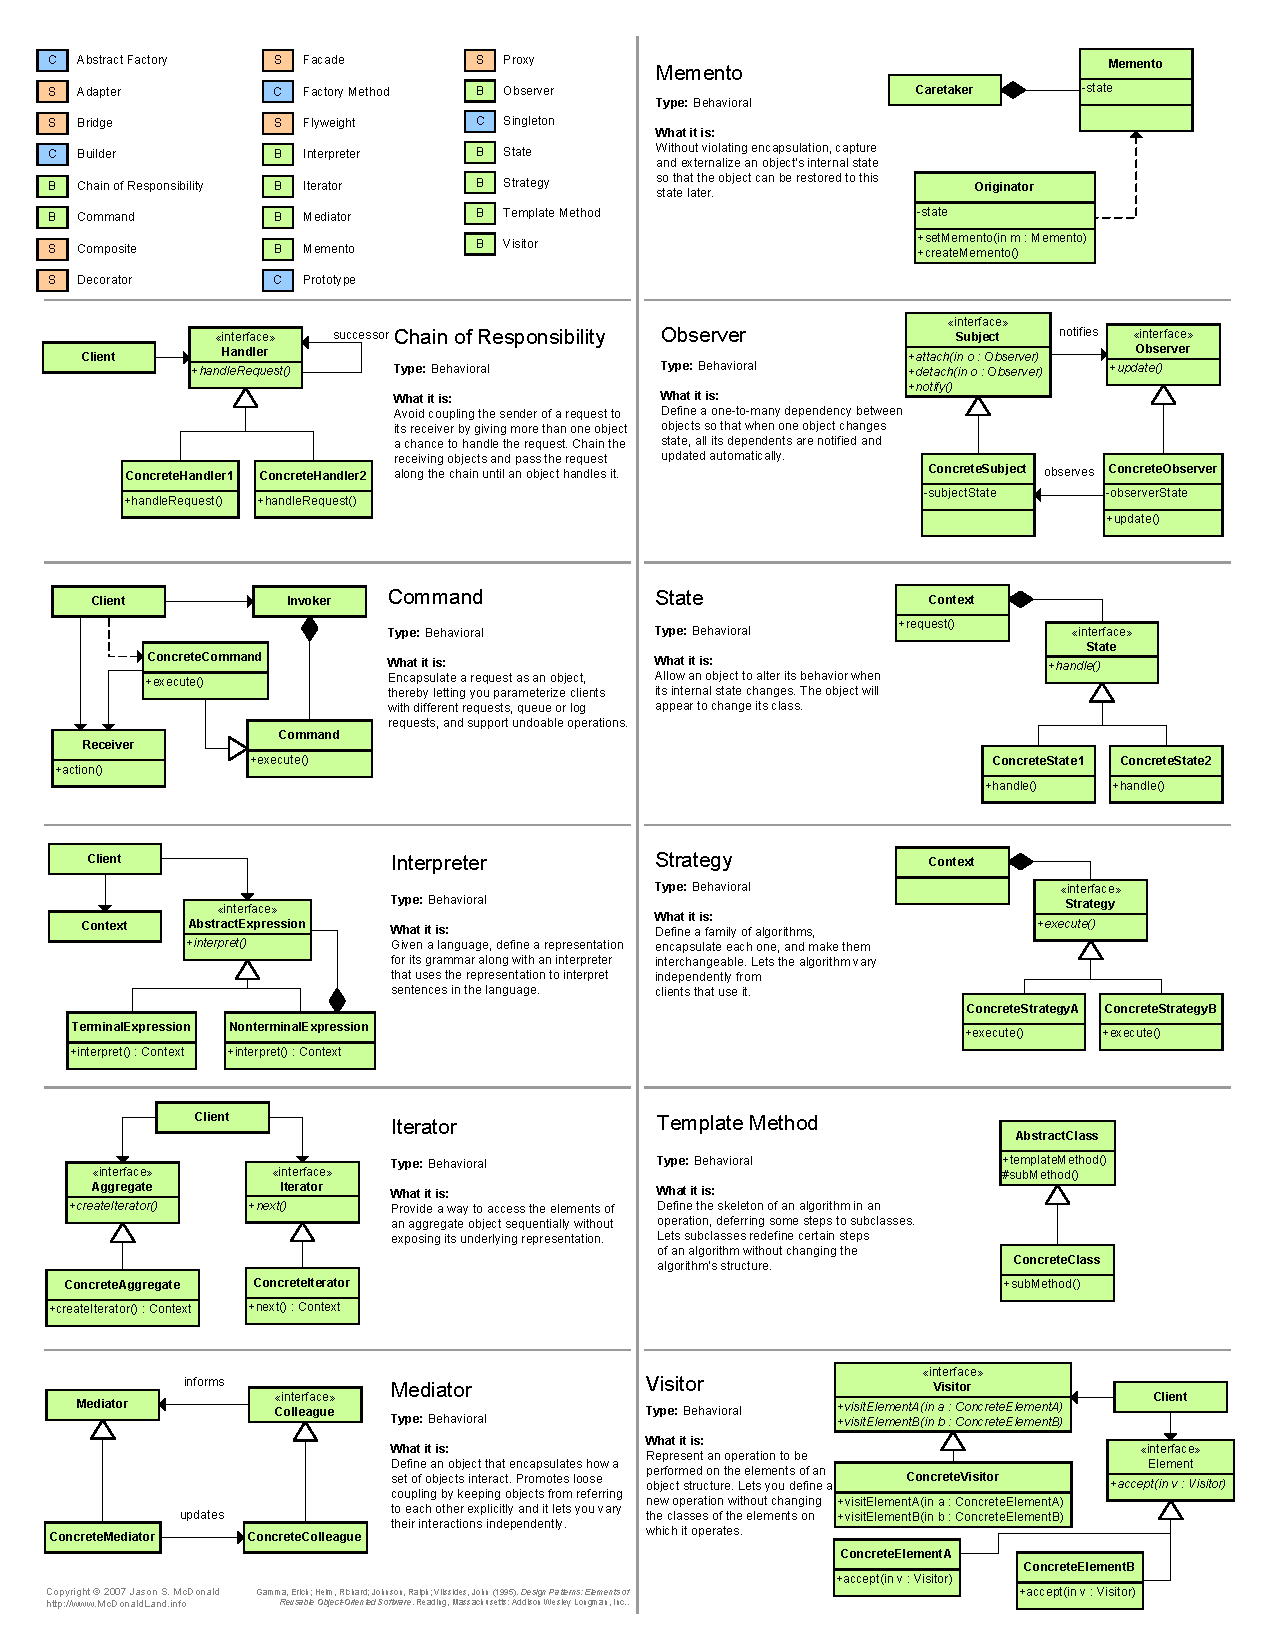
\includepdf[pages={1,2}]{./workshop-2/designpatternscard.pdf}
\end{appendices}

\begin{thebibliography}{9}

\bibitem{boehm}
  Boehm, B.; Turner, R., ''Observations on balancing discipline and agility'', Agile Development Conference, 2003.
  ADC 2003. Proceedings of the , vol., no., pp.32,39, 25-28 June 2003
  
\bibitem{larman}
Larman, Craig, ''Agile and Iterative Development: A Manager's Guide''.
Addison-Wesley, 2004.

\bibitem{checklist}
Gloger, Boris, ``Scrum Checklist'', 

\url{http://sict.moodle.aau.dk/file.php/797/General\_Course\_Materials/
literature/Scrum\_CheckList\_2011.pdf}, Set 10 Oktober 2013
\end{thebibliography}

\end{document}